\documentclass[tikz, border=5mm]{standalone}
\usepackage{amsmath}

\begin{document}
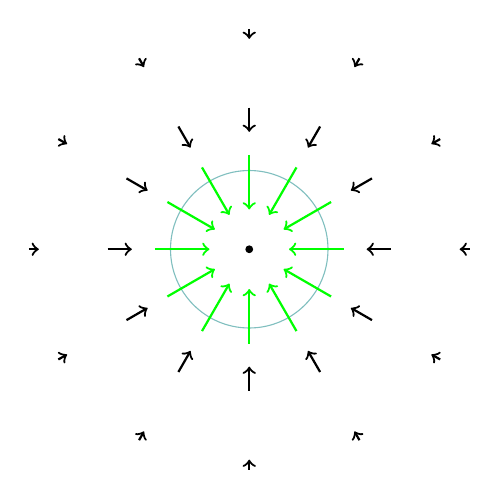
\begin{tikzpicture}
  % Paramètres
  \def\radius{1} % Rayon de la Terre (maintenant fixé à 1)
  \def\gSurface{9.81} % Accélération à la surface (m/s^2)
  \def\numAltitudes{3} % Nombre d'altitudes différentes
  \def\scaleFactor{0.1} % Facteur d'échelle pour les vecteurs (ajuster pour la visualisation)

  % Couleurs pour chaque altitude
  \colorlet{altitudeColor1}{red}
  \colorlet{altitudeColor2}{green}
  \colorlet{altitudeColor3}{blue}

  % Dessiner la Terre
  \draw[blue!50!green!50] (0,0) circle (\radius);
  \node at (0,0) [circle, fill, inner sep=1pt, color=black] {};

  % Fonction pour calculer l'accélération gravitationnelle relative à une altitude donnée
  \pgfmathdeclarefunction{relativeGravitationalAcceleration}{1}{%
    \pgfmathparse{1/(1+#1)^2}%
  }

  % Boucle sur les différentes altitudes
  \foreach \altitudeIndex in {1,4,9}
  {
    % Définir l'altitude relative pour cet indice
    \pgfmathsetmacro{\relativeAltitude}{\altitudeIndex * 0.2} % Ex: 0.2, 0.4, 0.6

    % Choisir la couleur pour cette altitude
    \ifcase\altitudeIndex
      \colorlet{currentAltitudeColor}{altitudeColor1} \or
      \colorlet{currentAltitudeColor}{altitudeColor2} \or
      \colorlet{currentAltitudeColor}{altitudeColor3} \else
      \colorlet{currentAltitudeColor}{black} % Couleur par défaut si plus de 3 altitudes
    \fi

    % Boucle sur les angles
    \foreach \angle in {0,30,60,90,120,150,180,210,240,270,300,330}
    {
      % Calcul de l'accélération gravitationnelle relative
      \pgfmathsetmacro{\relativeAcceleration}{relativeGravitationalAcceleration(\relativeAltitude)}

      % Calcul de la longueur du vecteur
      \pgfmathsetmacro{\vectorLength}{10*\relativeAcceleration * \scaleFactor}

      % Coordonnées du point de départ du vecteur
      \pgfmathsetmacro{\xStart}{(\radius + \relativeAltitude) * cos(\angle)}
      \pgfmathsetmacro{\yStart}{(\radius + \relativeAltitude) * sin(\angle)}

      % Dessiner le vecteur
      \draw[currentAltitudeColor, ->, thick] (\xStart,\yStart) -- ({(\radius + \relativeAltitude - \vectorLength) * cos(\angle)}, {(\radius + \relativeAltitude - \vectorLength) * sin(\angle)});
    }
  }
\end{tikzpicture}
\end{document}
